\documentclass[10pt,a4paper]{article}
\usepackage[margin=2.2cm]{geometry}
\usepackage{fontspec}
\usepackage{kotex}
\setmainfont{Apple SD Gothic Neo}
\setsansfont{Apple SD Gothic Neo}
\usepackage{amsmath,amssymb}
\usepackage{graphicx}
\usepackage{caption}
\usepackage[dvipsnames]{xcolor}
\usepackage[colorlinks=true,linkcolor=MidnightBlue,citecolor=MidnightBlue,
            urlcolor=MidnightBlue]{hyperref}
\usepackage{titlesec}
\titleformat{\section}{\large\bfseries}{\thesection}{0.6em}{}
\captionsetup{font=small,labelfont=bf}
\setlength{\parskip}{0.35em}
\setlength{\parindent}{0pt}
\usepackage{mdframed}
\newmdenv[linewidth=0.4pt,linecolor=gray!60,backgroundcolor=gray!5,
          innertopmargin=6pt,innerbottommargin=6pt,skipabove=8pt,skipbelow=8pt]{claimbox}
\newcommand{\claim}[2]{\begin{claimbox}\textbf{주장.} #1\par\smallskip
  \textcolor{gray!70}{\textbf{반증 조건.} #2}\end{claimbox}}

\title{\bfseries 챔피언 예측은 배치 함수다\\[2pt]
\large 격리 팔 자기시험의 실패가 캔 것 --- 그리고 `수리는 편향, 누적은 분산'}
\author{월드모델 실험실 · 노트 $849$ (부: $847$ 정정 $2$건 · $848$ 측정 전 수정)}
\date{2026-08-09}
\begin{document}\maketitle

\section{한 줄}

격리 팔($30$편 중 $3$편만 값 변경) 자기시험이 \textbf{실패했다} --- 비회복
$27$행의 순서가 보존되지 않았다. 원인 실측: F$18$ 의 \texttt{\_spec\_col}
(forms.py:$550$)이 \textbf{예측 배치 전체에 rankdata 를 거는 피처}라, $3$편의
venue 가 바뀌면 $30$편 전원의 설계행이 변한다. \textbf{챔피언 예측은 행
함수가 아니라 배치 함수다} --- 내 기제 주장과 티처 \#$14$ 의 `원리상 불가능'
논거가 같은 자기시험에서 함께 반증됐다(티처의 결론 자체는 코드로 생존 ---
증거만 교체).

\begin{figure}[t]\centering
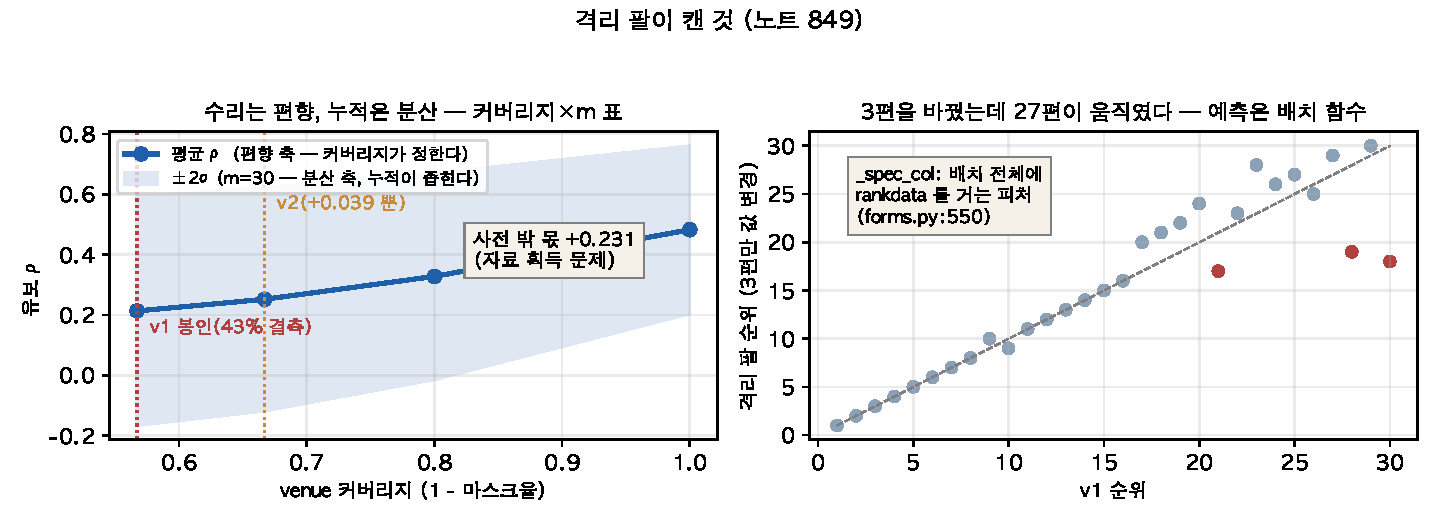
\includegraphics[width=0.97\textwidth]{figs/batchfn.pdf}
\caption{왼쪽: 커버리지$\times m$ 표 --- 평균(편향)은 커버리지 축, $\pm2\sigma$
(분산)는 $m$ 축이 정한다. 오른쪽: $3$편 변경이 $27$편을 움직였다.}
\end{figure}

\claim{\textbf{`수리는 편향을 지우고 누적은 분산을 줄인다' --- $847$ 의
`지렛대는 누적 $4.3$배'는 범주 오류였다.} between $\sigma$ $0.041$ 은 고정
마스크율에서의 뽑기 요동이지 커버리지 효과가 아니다 --- 커버리지 결손은
같은 사전을 쓰는 모든 봉인에 공통인 \emph{계통 편향}이라 편수로 안 사라진다.
커버리지$\times m$ 표(annex$4$)가 두 축을 가른다: 평균 $0.2129$(마스크
$43.3\%$) $\to 0.4822$(완전 관측), $2\sigma(m{=}30)$ $0.380 \to 0.278$.
그리고 이득 분해가 다음 수리의 주소를 바꿨다: \textbf{v$2$ 정규화 몫은
$+0.039$ 뿐이고 사전 밖 몫이 $+0.231$} --- 남은 일은 코드가 아니라 자료
획득($897$ 사전의 폭)이다.}
{봉인 간 합산에 코호트 효과 미결 등록(결정 규칙 포함): 배치 함수인 예측을
봉인별로 합산할 때 `봉인별 $\rho$ 가중평균'과 `전 코호트 한 배치 재예측
$\rho$'의 차가 봉인별 $2\sigma$ 의 절반을 넘으면 합산 규칙을 재사전등록한다.}

\section{부 --- 같은 사이클의 정정과 수정}

$847$ 정정 $2$건: v$2$ 는 회복 $3$편이 아니라 덮인 $30$편 전체를 재척도했다
(코드 사실 --- 캐스케이드 해명 철회), `$4.3$배' 범주 오류. $848$ 측정 전
수정(체크포인트 = 앵커 $1$행뿐인 상태에서): \texttt{MIN\_TRAIN}$=15$ 가
$n{=}10$ 격자점을 조용히 죽인다(티처 \#$14$) $\to$ 격자
$\{15,20,40,80,160\}$ · 릿지 팔 순위 목표 · 누출 표면 제거. $\Delta(n)$ 은
지금 배경에서 돈다 --- 판정은 다음 노트. 예측 채점 $3/4$(미스가 곧 발견).
GitHub 흐름 $9$회째. 판 $\rho$ $0.4710$ 그대로.

\end{document}
